\documentclass[11pt]{amsart}
\usepackage[T1]{fontenc}
\usepackage{lmodern,mathtools,tikz}
\usepackage[margin=28mm]{geometry}
\usepackage[hidelinks]{hyperref}
\usetikzlibrary{arrows.meta}
\newtheorem{theorem}{Theorem}
\newtheorem{proposition}[theorem]{Proposition}
\newcommand{\Cov}{\operatorname{Cov}}
\newcommand{\Tr}{\operatorname{Tr}}
\newcommand{\E}{\mathbb E}
\title[Replica seams and the Wilson thermal defect]{Replica Seams and the Weak-Coupling Yang--Mills Gap}
\date{anaxia research working note}
\keywords{Yang--Mills theory, thermal defect, replica seams}
\subjclass[2020]{Primary 81T13 (Yang--Mills theory).
Secondary 81T08 (constructive quantum field theory), 81T25 (lattice quantum
field theory), 81T27 (continuum limits), 81T28 (thermal quantum field theory).}

\begin{document}
\begin{abstract}
Two replica seams express the Wilson thermal defect as an exact connected covariance. We prove a sharp finite-volume contraction and quantify the uniform response estimate needed for a weak-coupling mass gap.
\end{abstract}
\maketitle

\section{The estimate at issue}

The Clay problem asks for a nontrivial continuum quantum Yang--Mills theory on
\(\mathbb R^4\) with a positive mass gap for every compact simple gauge group
\cite{JW}. The one-scale argument of \cite{OneScale} gives a conditional path
from finite rectangular Wilson partition functions to a continuum spectral
gap. Its weak-coupling estimate has to hold at the same bare coupling for
both temporal periods and for every rectangle in the stated range.

Let \(Z_\beta(s,T)\) be the Wilson partition function at bare coupling
\(\beta\), on a spatial torus with integer sides \(s=(s_1,s_2,s_3)\) and
periodic time \(T\ge3\). Write \(V=\prod_i s_i\) and set
\[
 \Psi_\beta(s,T)=2\log Z_\beta(s,T)-\log Z_\beta(s,2T).
\]
Our calculations isolate a precise response estimate that would yield
the uniform seed. It remains to prove that estimate in the interacting
weak-coupling theory.

\section{The finite Wilson identity}

Replica gluing is used in lattice gauge entropy calculations \cite{Replica}.
Here both switches act on whole spatial layers. Take two time-\(T\)
sheets. At each of two temporal cuts \(a,b\), introduce
independent straight and swapped bundles of links. Each bundle joins every
spatial site to the same site on the next slice. A straight link preserves
its sheet label, and a swapped link changes it. A temporal plaquette at a
cut uses both time edges from one matching and the top spatial edge on
the corresponding sheet. The loop closes, so its Wilson term is gauge
invariant under independent transformations at every vertex.\footnote{All
 link variables, including inactive links, are integrated against normalized
 Haar probability measure. An inactive bundle therefore contributes exactly
 one. A constant shift of the ordinary action per spacetime site cancels
 from \(\Psi_\beta\).}

Let \(S_c^0,S_c^1\) be the Wilson sums at cut \(c\) for the two matchings,
including the coupling, and write \(\Delta_c=S_c^1-S_c^0\).
Keep all plaquettes off the cuts and add
\(S_a^0+u\Delta_a+S_b^0+v\Delta_b\), where \(0\le u,v\le1\).
Let \(F(u,v)\) denote the resulting log partition function, with
\(\Cov_{u,v}\) computed in its normalized probability measure.

\begin{theorem}
For every finite box and every finite coupling,
\[
 \Psi_\beta(s,T)
   =\frac12\int_0^1\!\!\int_0^1\Cov_{u,v}(\Delta_a,\Delta_b)\,du\,dv.
\]
If \(A_x,B_y\) collect the corresponding cut differences based at spatial
sites \(x,y\), then
\[
 \frac{\Psi_\beta(s,T)}{V}
   =\frac12\int_0^1\!\!\int_0^1
      \sum_y\Cov_{u,v}(A_0,B_y)\,du\,dv.                   \tag{1}
\]
\end{theorem}

\begin{proof}
At an endpoint, following the active time edges around the time circle
gives the composition of the two matchings (Figure~\ref{fig:seams}). Equal cut labels give two
cycles of length \(T\); opposite labels give one cycle of length \(2T\).
The relabeling preserves the spatial links and plaquettes on each time
slice. Inactive bundles integrate to one. Thus \(F(0,0)=F(1,1)=2\log
Z_\beta(s,T)\) and \(F(1,0)=F(0,1)=\log Z_\beta(s,2T)\).
The finite exponent is bounded on the compact product of groups, so
differentiation under the integral gives
\(\partial_u\partial_v F=\Cov_{u,v}(\Delta_a,\Delta_b)\).
Integrate over the unit square and use the four endpoint values.
The second identity follows by summing the site covariances and using
spatial translation invariance.
\end{proof}

\begin{figure}[ht]
\centering
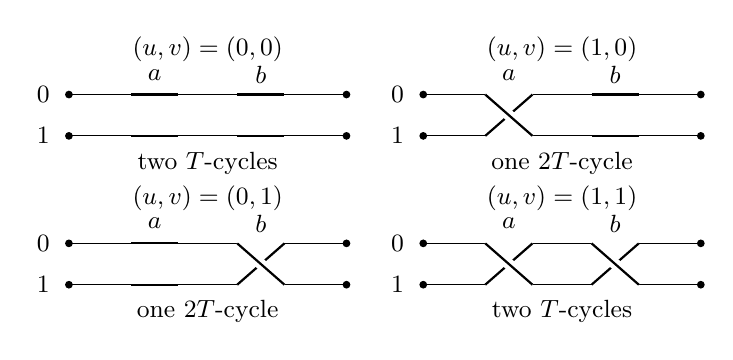
\begin{tikzpicture}[x=.75cm,y=.7cm, every node/.style={font=\small}]
\foreach \xo/\yo/\u/\v/\cap in {
  0/2.7/0/0/{two \(T\)-cycles},6/2.7/1/0/{one \(2T\)-cycle},
  0/0/0/1/{one \(2T\)-cycle},6/0/1/1/{two \(T\)-cycles}} {
  \begin{scope}[shift={(\xo,\yo)}]
    \node at (2.35,2.02) {\((u,v)=(\u,\v)\)};
    \node[anchor=east] at (-.16,1.2) {\(0\)};
    \node[anchor=east] at (-.16,.45) {\(1\)};
    \foreach \h in {.45,1.2} {
       \draw (0,\h)--(1.05,\h) (1.85,\h)--(2.85,\h) (3.65,\h)--(4.7,\h);
       \fill (0,\h) circle (1.4pt) (4.7,\h) circle (1.4pt);
    }
    \ifnum\u=0
       \draw[thick] (1.05,.45)--(1.85,.45) (1.05,1.2)--(1.85,1.2);
    \else
       \draw[thick] (1.05,.45)--(1.85,1.2);
       \draw[thick,preaction={draw=white,line width=4pt}] (1.05,1.2)--(1.85,.45);
    \fi
    \ifnum\v=0
       \draw[thick] (2.85,.45)--(3.65,.45) (2.85,1.2)--(3.65,1.2);
    \else
       \draw[thick] (2.85,.45)--(3.65,1.2);
       \draw[thick,preaction={draw=white,line width=4pt}] (2.85,1.2)--(3.65,.45);
    \fi
    \node at (1.45,1.56) {\(a\)};
    \node at (3.25,1.56) {\(b\)};
    \node at (2.35,-.04) {\cap};
  \end{scope}
}
\end{tikzpicture}
\caption{The active time connections at the four corners. In each panel,
 identify the left and right endpoints with the same row label. A crossing
 changes sheets without joining the two drawn edges.}
\label{fig:seams}
\end{figure}

There is also a bounded-observable form. Give the two matching labels
\(\sigma_a,\sigma_b\in\{-1,1\}\) equal independent priors before weighting
by the Wilson exponent. Integrate all active and inactive links in this
enlarged ensemble. Each label has mean zero by the corner values and
\(\E[\sigma_a\sigma_b]=\tanh(\Psi_\beta/2)\).
Given the links the labels are independent, with conditional means
\(m_c=\tanh(\Delta_c/2)\). Consequently
\[
 \tanh(\Psi_\beta/2)=\Cov(m_a,m_b).                         \tag{2}
\]
The responses in (2) are bounded in magnitude by one. Each depends on its
entire cut, and the marginal link measure contains the corresponding
full-cut weights \(e^{S_c^0}+e^{S_c^1}\).

\section{An optimal transfer bound}

For the Wilson application at \(\beta\ge0\), \(Z_\beta(s,T)\) is the
trace of the \(T\)-th power of the Wilson transfer operator on its
gauge-invariant Hilbert space, using the trace normalization of
\cite[Lemma 7.3]{OneScale}. Use a positive self-adjoint transfer operator
with a simple leading eigenvalue and assume its \(T\)-th power has finite
trace. Let \(x_j\) be the excited eigenvalue
ratios raised to the \(T\)-th power. Set \(D=\sum_jx_j\),
\(E=\sum_jx_j^2\), \(F_4=\sum_jx_j^4\), and \(a=e^{\Psi(T)}-1\).
Here \(\Psi(T)\) is computed from the transfer traces.\footnote{Dividing
 the transfer operator by its leading eigenvalue changes the log trace
 by a term linear in time, which cancels from the defect.}

\begin{proposition}
If \(0\le a<1\), then
\[
 D\le\frac{a}{1+\sqrt{1-a^2}},\qquad
 e^{\Psi(2T)}-1\le\frac{a^2}{2-a^2}.
\]
For \(0<a<1\), both bounds are attained with a single positive excited
weight. For \(a=0\), all excited weights vanish.
\end{proposition}

\begin{proof}
Put \(R=1+a=(1+D)^2/(1+E)\). From \(E\le D\) we get \(D\le a\).
Since \(E\le D^2\), \(a\ge2D/(1+D^2)\), giving the first bound. Write its
right-hand side as \(d_*\). If \(D=0\), the second bound is immediate.
Otherwise Jensen's inequality with weights \(x_j/D\) gives
\(F_4\ge E^3/D^2\), so
\[
 e^{\Psi(2T)}\le U(D)=\frac{(1+E)^2}{1+E^3/D^2},
 \qquad E=(1+D)^2/R-1.
\]
For fixed \(R\), the interval \(\sqrt R-1\le D\le d_*\) has
\(0\le E\le D^2\). Multiplying the logarithmic derivative of \(U\) by
\((1+D)(D^2+E^3)\) gives \(4D^2-6E^2+2E^3/D\).
On that interval \(E^2(3-E/D)\le D^4(3-D)\le2D^2\), so
\(U\) is nondecreasing. At \(D=d_*\), \(E=d_*^2\) and
\(U(d_*)-1=2d_*^2/(1+d_*^4)=a^2/(2-a^2)\). A single weight \(d_*\)
realizes every equality.
\end{proof}

\begin{figure}[ht]
\centering
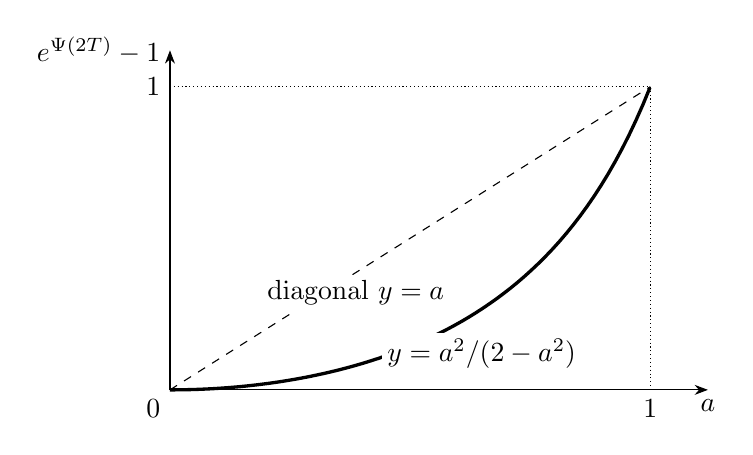
\begin{tikzpicture}[x=6.1cm,y=3.85cm,>=Stealth]
\draw[->] (0,0)--(1.12,0) node[below] {\(a\)};
\draw[->] (0,0)--(0,1.12) node[left] {\(e^{\Psi(2T)}-1\)};
\draw[densely dotted] (0,1)--(1,1)--(1,0);
\draw[dashed] (0,0)--(1,1);
\draw[very thick,samples=70,domain=0:1] plot (\x,{\x*\x/(2-\x*\x)});
\node[anchor=west,fill=white,inner sep=2pt] at (.19,.32) {\(\text{diagonal } y=a\)};
\node[anchor=west,fill=white,inner sep=2pt] at (.44,.12) {\(y=a^2/(2-a^2)\)};
\node[below left] at (0,0) {\(0\)};
\node[below] at (1,0) {\(1\)};
\node[left] at (0,1) {\(1\)};
\end{tikzpicture}
\caption{The sharp time-doubling bound on a single fixed box. The solid
curve is attained by one excited weight.}
\label{fig:contraction}
\end{figure}

\section{The uniform requirement}

Suppose every spatial side lies in \([2T,40T)\) and
\(\Psi_\beta(s,T)\le V/(13{,}510{,}000\,T^3)\).
Then \(\Psi\le u=32/6755\). Writing \(Z_{\rm vac}(T)=1+D\), we have
\[
 \log Z_{\rm vac}(T)
 =\tfrac12\bigl(\Psi+\log(1+E)\bigr)
 \le \tfrac12\left(1+\frac{u}{(1-u)^2}\right)\Psi,
\]
because \(E\le (e^\Psi-1)^2\) and \(e^\Psi-1\le\Psi/(1-\Psi)\).
The coefficient on \(V/T^3\) is therefore at most \(1/26{,}880{,}000\),
the smaller-window pressure seed in the one-scale refinement \cite{Ann}.
The exact ratio of the obtained coefficient to the required one is
\(2906552896/2907784899\). With the matching continuum hypothesis (W) of
\cite{OneScale}, the third row of \cite{Ann} then gives
\(\Delta\ge t_0^{-1}\log(80724/80645)\).

In the quantifiers of \cite[Theorem F]{OneScale}, a sufficient input is the
following. For some \(t_0>0\) and all sufficiently large \(p\), for every
\(N\ge N_0(p)\) select \(3\le T\le Nt_0\). At the same coupling
\(\beta_{N,p}\) for every rectangle in the window, prove
\[
 \int_0^1\!\!\int_0^1 \sum_y
         \Cov_{u,v}(A_0,B_y)\,du\,dv
       \le \frac{2}{13{,}510{,}000\,T^3}.                 \tag{3}
\]
For example, put the cuts at cyclic separation \(d=\lfloor T/2\rfloor\).
A bound
\[
 |\Cov_{u,v}(A_0,B_y)|\le
 C b^{-6}e^{-m(d+\operatorname{dist}_1(0,y))/b}
\]
with cutoff-independent \(C,m>0\) and \(b\ge1\) would give
\[
 \frac{T^3\Psi}{V}\le \frac C2 (1+2/m)^3 e^{m/2}(T/b)^3e^{-mT/(2b)}.
\]
Indeed each periodic spatial coordinate contributes at most
\(1+2/(e^{m/b}-1)\le b(1+2/m)\) to the sum in (1).
This suffices if the required large ratio \(T/b\) is reached within the
available physical time window. The estimate must control the amplitude
as well as the range of correlations.

\section{A Gaussian check}

On a spatial cube of side \(2T\), the first nonzero nearest-neighbor
massless oscillator has energy
\(E_1=2\operatorname{arsinh}(\sin(\pi/(2T)))\le\pi/T\).
Keep its even occupation numbers, with vacuum energy zero.
For \(q=e^{-2TE_1}\), the traces at \(T,2T\) are \(1/(1-q)\) and
\(1/(1-q^2)\). Hence its defect is
\(\log((1+q)/(1-q))\ge2q>2/3^7>8/13{,}510{,}000\).
The last term is the target on this cube. Thus a comparison to the
massless quadratic theory needs control of the terminal fluctuations.
Known temporal-cluster cancellation from the strong-coupling character
expansion \cite{LMP} applies in its small-coupling-parameter regime.
At weak bare coupling, matching the nonwinding coefficients at the
two periods and bounding the terminal contributions would require
additional estimates.

There is a separate obstruction to deducing the thermal bound solely from
convergence of a monitored algebra of normalized correlations. For any
transfer family at lattice spacing \(a_0\), tensor the transfer operator
with \(\operatorname{diag}(1,e^{-a_0\epsilon_{a_0}})\), and tensor every
monitored observable with the identity. Each normalized trace correlation
is unchanged by exact cancellation of the extra factor. At \(T a_0=t\)
the additional defect is
\[
 \log\frac{(1+e^{-t\epsilon_{a_0}})^2}{1+e^{-2t\epsilon_{a_0}}}
 \ \longrightarrow\ \log 2
 \qquad (\epsilon_{a_0}\to0).
\]
This transfer example identifies the state-counting information absent
from the monitored correlations. It concerns an auxiliary tensor factor.
The continuum assessment \cite{Assessment} similarly distinguishes its
reconstruction results from the spectral gap question.
The Clay conclusion still requires (3), or another uniform gap estimate,
and a matching nontrivial continuum construction for the groups in its
statement.

\section*{Data availability}

The \href{https://github.com/anaxia-research/anaxia}{anaxia repository}
contains the \href{https://github.com/anaxia-research/anaxia/tree/main/anaxia/ann}{\texttt{ann} agent workbench},
its \href{https://github.com/anaxia-research/anaxia/blob/main/docs/ANN.md}{replay instructions},
and the \href{https://github.com/anaxia-research/anaxia/blob/main/research/weak-coupling-seams/evidence.json}{campaign evidence summary}.
The weak-coupling campaign scheduled all 10,000 agent profiles, one task
per profile, with at most 24 workers active at a time. All 10,000 tasks
completed across 13 prescribed routes. Rational replays checked the
replica endpoint algebra, the single-excitation equality, multilevel
contraction, and the numerical Gaussian comparison. The campaign
used deterministic workers.

A subsequent focused run completed 192 deterministic tasks across six
routes, including the connected-activity and conditional block entropy
constructions. Its \href{https://github.com/anaxia-research/anaxia/blob/main/research/weak-coupling-seams/constructions-evidence.json}{evidence summary}
and \href{https://github.com/anaxia-research/anaxia/blob/main/docs/ANN-YANG-MILLS-CONSTRUCTIONS.md}{proof notes}
document those additional routes.

An exhaustive run checked \(575{,}704\) grid cases for positive transfer
spectra with up to four excited weights and denominators \(4\) through \(35\).
All \(4{,}176\) cases in the small-defect regime passed the exact
time-doubling test, with \(592\) equalities. The
\href{https://github.com/anaxia-research/anaxia/blob/main/research/weak-coupling-seams/exhaustive-evidence.json}{exhaustive evidence}
concerns these finite rational spectra.

\section*{Acknowledgments}

We credit \href{https://github.com/creelie}{Deep Bhattacharjee}, creator of
\href{https://github.com/anaxia-research/anaxia}{anaxia}, for initiating the project and directing the development
of its \href{https://github.com/anaxia-research/anaxia/tree/main/anaxia/ann}{\texttt{ann} workbench}
used for these research campaigns.

\begin{thebibliography}{9}
\bibitem{JW} A.~Jaffe and E.~Witten, \emph{Quantum Yang--Mills Theory},
Clay Mathematics Institute. \url{https://www.claymath.org/wp-content/uploads/2022/06/yangmills.pdf}
\bibitem{OneScale} D.~Bhattacharjee, U.~Bhattacharya, J.~M.~Lockwood,
T.~Romanov, I.~J.~Sessford, and S.~S.~Roy,
\emph{The Yang--Mills Mass Gap from One Bound at One Scale},
Theorem F and Proposition 7.57, 2026.
\url{https://www.preprints.org/manuscript/202611.1282}
\bibitem{Ann} anaxia research,
\emph{A wider pressure allowance in the conditional Yang--Mills criterion}.
\url{https://github.com/anaxia-research/anaxia/blob/main/docs/YANG-MILLS-ONE-SCALE.md}
\bibitem{Replica} T.~Rindlisbacher, N.~Jokela, A.~P\"onni, K.~Rummukainen,
and A.~Salami, \emph{Improved lattice method for determining entanglement
measures in SU(N) gauge theories}, PoS(LATTICE2022)031.
\url{https://arxiv.org/abs/2211.00425}
\bibitem{LMP} J.~Langelage, G.~M\"unster, and O.~Philipsen,
\emph{Strong coupling expansion for finite temperature Yang--Mills theory
in the confined phase}, JHEP 07 (2008), 036. \url{https://arxiv.org/abs/0805.1163}
\bibitem{Assessment} Yang--Mills group, \emph{Validation of the OpenAI
Yang--Mills construction}, 10 November 2026.
\url{https://alexisdpc.github.io/yang-mills/references/assessment-1-2026-11-10.pdf}
\end{thebibliography}
\end{document}
